\documentclass[a4paper]{iutvexam}
% compile-latex options:--jobname controle20161201
% compile-latex options:--jobname correction20161201
\usepackage{textcomp,booktabs}
\usepackage{tikz}
\usetikzlibrary{calc}
\usepackage{listings}
\lstset{basicstyle=\ttfamily,
  showstringspaces=false,
  commentstyle=\itshape,
  keywordstyle=\bfseries,
  literate={á}{{\'a}}1 {ã}{{\~a}}1 {é}{{\'e}}1 
}

\title{Contrôle 2}
\date{1/12/2016}
\begin{document}
\conditions{ Vous disposez de 2 heures pour faire ce contrôle. Aucun
  document autorisé, à part votre annexe qui aura été rédigée de façon
  manuscrite par vos soins sur une feuille A4 recto. Toute tentative de
  communication avec un voisin ou l'extérieur peut être
  sanctionnée. Toutes les réponses doivent être faites sur l'énoncé. La
  taille de la réponse attendue dépend de la taille allouée pour
  répondre. }
\begin{questions}
  \titledquestion{Mémoire}

  Dans un processeur, la règle technologique (classique) suivante est
  toujours respectée:
  \begin{quote}
    les adresses d'une donnée (variable ou champ d'une variable de type
    \texttt{struct}) doivent toujours être un multiple de la taille de
    la variable si sa longueur en octets est moins qu'un mot-machine, et
    un multiple du mot-machine sinon.
  \end{quote}

  Dans le cas qui nous intéresse d'un processeur 32 bits, le mot-machine
  est un \texttt{int} de (évidemment) 32 bits, le \texttt{short int} est
  de 2 octets. Une adresse occupe un mot-machine aussi. L'ordinateur 32
  bits est un ordinateur \texttt{little endian} (les valeurs sur
  plusieurs octets sont stockées avec les poids faibles dans les petites
  adresses).

  Une structure \texttt{struct bidule} est définie par:

\begin{verbatim}
typedef struct bidule {  short int longueur; char type; char* adresse; }
\end{verbatim}

  Une variable \texttt{a} qui est un \texttt{struct bidule}, commence à l'adresse \texttt{0x8004} et est suivie d'une variable \texttt{b} de même type.


  La structure \texttt{a} a été initalisée avec les valeurs \verb|{1023, 45, 0x8000}|, sachant que la chaîne \texttt{c} à l'adresse \texttt{0x00008000} était "A0" (dans le code ASCII en hexadécimal: 0x41 et 0x30).

  Les schémas ci-dessous peuvent être plus grands que nécessaires. Ou pas.

  \begin{parts}
    \part[1] Représentez sur le schéma ci-dessous les cases mémoires occupées par la variable \texttt{a} et les cases mémoires occupées par la variable \texttt{b}.
    \part[1] Représentez sur le même schéma les cases mémoires occupées par chacun des champs des variables \texttt{a} et \texttt{b} (mettez le nom des champs dans les cases).

    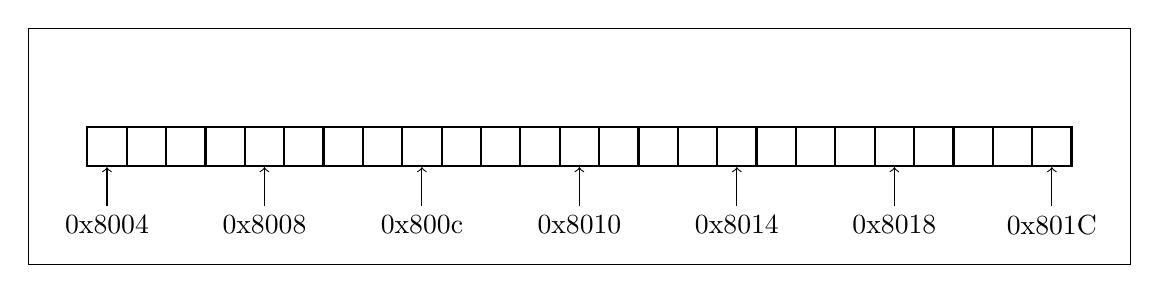
\begin{tikzpicture}
      \foreach \x in {4,5,...,28}{
        \node (a\x) [rectangle,draw=black,thick, minimum size=5mm] at (\x/2,0){};
      }
      \foreach \x/\y in {4/04,8/08,12/0c,16/10,20/14,24/18,28/1C}{
        \node (b\x) at ($ (a\x)+(0,-1) $) {0x80\y};
        \draw [->] (b\x) to (a\x);
      }
      \draw ($ (a4)+(-1,-1.5) $) rectangle ($ (a28)+(1,1.5) $);
    \end{tikzpicture}
    \part[1] Dans le schéma ci-dessous, représentez le contenu des cases mémoires en hexadécimal (ou en ASCII à votre choix) concernées par la chaîne \texttt{c}.
    \part[1] Dans le même schéma ci-dessous, représentez le contenu des cases mémoires en hexadécimal concernées par la variable \texttt{a}.

    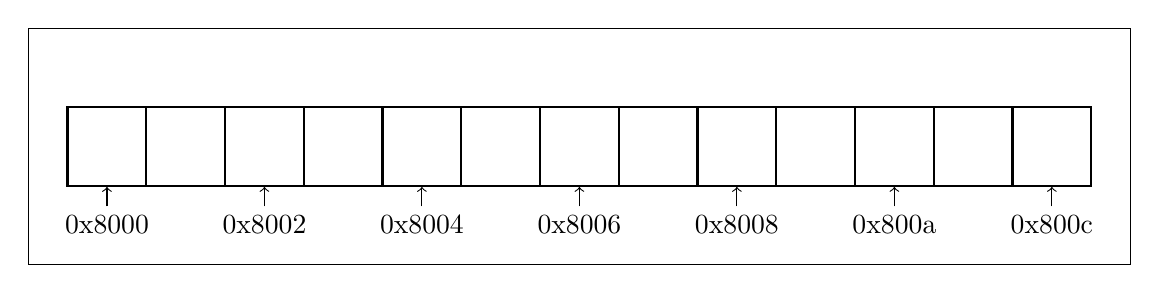
\begin{tikzpicture}
      \foreach \x in {0,1,...,12}{
        \node (a\x) [rectangle,draw=black,thick, minimum size=10mm] at (\x,0){};
      }
      \foreach \x/\y in {0/00,2/02,4/04,6/06,8/08,10/0a,12/0c}{
        \node (b\x) at ($ (a\x)+(0,-1) $) {0x80\y};
        \draw [->] (b\x) to (a\x);
      }
      \draw ($ (a0)+(-1,-1.5) $) rectangle ($ (a12)+(1,1.5) $);
    \end{tikzpicture}
    \part[1] Pour un ordinateur \emph{64 bits}, quelle est la taille d'un \texttt{struct bidule} ?
    \begin{solutionordottedlines}[.25in]%
      Alignement, taille des adresses : une structure prendrait
      maintenant 2 fois 64 bits.
    \end{solutionordottedlines}
  \end{parts}
  \newpage

  \titledquestion{Données}

  \begin{parts}
    \part[1] Expliquez deux façons possibles de coder la chaîne de caractère \texttt{"MÉROU"} dans divers environnements (il en existe au moins quatre, deux suffisent). Faites un schéma pour les deux.
    \begin{solutionorbox}[1in]%
      On peut soit faire varier l'encodage (ils n'ont pas besoin de connaître les codes exacts, juste expliquer et bien), soit le stockage (caractère nul terminal ou longueur puis données). UTF-8, ISO-latin d'un côté, caractère nul terminal ou valeur 5 en préfixe.
    \end{solutionorbox}

    \part[1] Un echantillon de son a été enregistré en stéréo pendant 5 secondes au format PCM: entête de 6 mots de 32 bits, avec codage des données à la suite de l'entête. La fréquence d'échantillonnage est de 8000 Hz, en \textmu-law (8 bits par échantillon) stéréo. Quelle est la taille du fichier final (tout compris) ?
    \begin{solutionordottedlines}[.25in]%
      8000*2*5 octets pour les données, 6*4 pour l'entête : 80024 octets.
    \end{solutionordottedlines}

    \part[1] Donnez un format le plus adapté pour ces trois images:\\
    \begin{center}
      \begin{tabular}{c|c|c}
        \includegraphics[width=.25\linewidth]{img/ctrl/lord-attack-mace.png} &
        \includegraphics[width=.25\linewidth]{img/ctrl/PythagoreanTreeB6.pdf} &
        \includegraphics[width=.25\linewidth]{img/ctrl/kitten.jpg}
      \end{tabular}
    \end{center}
    \begin{solutionordottedlines}[.25in]%
      PNG, Vectoriel (ici c'est un PDF), JPG
    \end{solutionordottedlines}

    \part[1] Donnez une valeur plausible au «~format HTML~» pour les couleurs suivantes : bleu, jaune, violet foncé, rose très pâle.
    \begin{solutionordottedlines}[.25in]%
      0000FF, FFFF00, 400040, FFA0A0. On cherchera pour les deux derniers la bonne tendance plutôt qu'une valeur exacte: le violet c'est du rouge et du bleu en proportion à peu près égale, foncé donc pas trop lumineux ; le rose pâle, c'est du rouge mélangé avec du blanc.
    \end{solutionordottedlines}
    
    \part[1] On veut compresser des séquences de bit selon la méthode de
    compression RLE. On va utiliser les données suivantes:
    \begin{itemize}
    \item On commence toujours par coder une série de 0 (éventuellement de longueur 0 si le premier bit est un 1);
    \item On code sur 4 bits les longueurs de séquence ; si on dépasse la longueur maximale, on met une séquence de longueur nulle de l'autre bit, puis on recommence.
    \end{itemize}
    Sur ces hypothèses, le codage de la séquence
    000000111100000000001...(20 fois 1 au total)...1 soit 03C00FFFFF
    s'écrit donc 6,4,3,1,1,1,4,15,0,5 donc 64AF05.

    Sur le même principe, donnez la compression RLE de la séquence de
    bits écrite en hexadécimal FF801FC.

    Est-ce que la compression RLE compresse toujours ? Si oui, à quel
    pourcentage maximum ? Sinon, donnez un contre-exemple
    \begin{solutionordottedlines}[.5in]%
      FF801FC=9,10,7,2 soit 09A72. Ici on compresse bien, mais ce n'est
      pas toujours le cas, par exemple A donne 01111 (+400\%).
    \end{solutionordottedlines}
  \end{parts}

  \newpage

  \titledquestion{Système}

  \begin{parts}

    \part[1] Pourquoi un processus a-t-il forcément un parent ? Dites comment il est créé.
    \begin{solutionordottedlines}[.75in]%
      La création d'un processus se fait par duplication/clonage d'un
      processus existant par l'appel système \texttt{fork}. Le processus
      qui subit le clonage devient alors le processus parent du clone.
    \end{solutionordottedlines}

    \part[1] Remplissez le tableau en indiquant pour chaque droit à
    quelle(s) action(s) il correspond dans le cas d'un fichier et d'un
    répertoire.
    \begin{center}
      \Large
      \begin{tabular}{p{4cm}cc}\toprule
        & pour un fichier &  pour un répertoire\\\midrule
        droit \texttt{r} & \hspace*{4cm} & \hspace*{4cm} \\
        droit \texttt{w} & \hspace*{4cm} & \hspace*{4cm} \\
        droit \texttt{x} & \hspace*{4cm} & \hspace*{4cm} \\\bottomrule
      \end{tabular}
    \end{center}
    \begin{solution}%
      lecture/modification/exécution et listing/suppression-création/traversée
    \end{solution}

    \part[1] Un fichier \texttt{FICHE} est lisible, exécutable et
    modifiable par tout le monde. On veut le rendre lisible par tout son
    groupe, modifiable par soi uniquement, et interdit à tous les autres
    ; il n'est pas exécutables. Donnez les deux formes de commandes
    (symbolique et numérique) qui permettent de rendre ceci possible.
    \begin{solutionordottedlines}[.5in]%
      \verb|chmod o-rwx,g-wx,u-x FICHE| ou \verb|chmod 640 FICHE|
    \end{solutionordottedlines}

    \part[1] Résumez les principales différences entre un script et un programme exécutable.
    \begin{solutionordottedlines}[.75in]%
      Un script est interprété ligne par ligne par \emph{un
        interpréteur}, alors que l'exécutable est obtenu par
      \emph{compilation} d'un code source. Les performances sont moins
      bonnes, mais c'est plus universel (pas de recompilation).
    \end{solutionordottedlines}
  \end{parts}

  \titledquestion{Shell}

  Un répertoire \texttt{etud} contient des fichiers qui portent des
  numéros d'étudiants du modèle \texttt{ANNEE-IDENTIFIANT.txt} (par
  exemple \texttt{2016-adZAHU.txt}). Chaque fichier contient ainsi une
  fiche étudiant avec des informations le concernant. Il comporta ainsi
  des lignes de données simples, comme par exemple \texttt{nom:Dubacq}
  ou \texttt{inscription:payée} (une seule ligne pour chaque clé
  maximum).

  Vous êtes dans le répertoire qui contient \texttt{etud}. Vous donnerez
  vos réponses sous forme de scripts courts ou d'unilignes (scripts en
  une ligne ; que vous pourriez taper directement dans le terminal,
  donc).

  Vous pouvez aussi écrire vos scripts en deux ou trois colonnes si
  l'espace alloué n'est pas suffisant.

  \begin{parts}
    \part[1] Déplacez tous les dossiers d'une année passée en paramètre dans un répertoire \texttt{archivage} qui est à peut-être à créer.
    \begin{solutionordottedlines}[.75in]%
      \begin{lstlisting}[language=bash,caption={bash version}]
        #!/bin/bash
        mkdir -p archivage
        cp etud/$1-* archivage/ # $1 est le parametre
      \end{lstlisting}
    \end{solutionordottedlines}

    \part[1] Faites un programme qui vérifie toutes les 5 secondes si le
    fichier \texttt{verrouillage} existe, et ne s'arrête que s'il
    n'existe plus (il affichera une ligne \texttt{"Attente..." sinon} et
    recommencera à attendre)
    \begin{solutionordottedlines}[1in]%
      \begin{lstlisting}[language=bash,caption={bash version}]
        #!/bin/bash
        while [ -f verrouillage ]; do
        echo "Attente..."
        sleep 5
        done
      \end{lstlisting}
    \end{solutionordottedlines}

    \newpage

    \part[1] Mettez dans une variable A le nombre de fichiers d'étudiants inscrits en 2016.
    \begin{solutionordottedlines}[.75in]%
      \begin{lstlisting}[language=bash,caption={bash}]
        #!/bin/bash
        A=$(ls etud/2016*|wc -l) # $A 
      \end{lstlisting}
    \end{solutionordottedlines}

    \part[1] Comptez les étudiants inscrits en 2016 en affichant
    \texttt{Nombre d'étudiants en 2016: 257} (ou autre valeur). S'il n'y
    en pas, affichez \texttt{Aucun étudiant en 2016} (vous pouvez réutiliser la question ci-dessus).
    \begin{solutionordottedlines}[1.75in]%
      \begin{lstlisting}[language=bash,caption={bash}]
        #!/bin/bash
        A=$(ls etud/2016*|wc -l)
        if [ $A -eq 0 ]; then
        echo "Aucun étudiant en 2016"
        else
        echo "Nombre d'étudiants en 2016: $A" # $A plus haut
        fi
      \end{lstlisting}
    \end{solutionordottedlines}

    \part[1] Comptez les étudiants inscrits en 2016 en affichant \texttt{Nombre d'étudiants en 2016: 257} (ou autre valeur). S'il n'y en pas, affichez \texttt{Aucun étudiant en 2016}
    \begin{solutionordottedlines}[1.25in]%
      \begin{lstlisting}[language=bash,caption={bash}]
        #!/bin/bash
        A=$(wc -l etud/2016*)"
        if [ $A -eq 0 ]; then
        echo "Aucun étudiant en 2016"
        else
        echo "Nombre d'étudiants en 2016: $A" # $A plus haut
        fi
      \end{lstlisting}
    \end{solutionordottedlines}

    \part[1] Comptez les fichiers d'apprentis (ligne \texttt{type:apprenti}) en affichant \texttt{Nombre d'apprentis: 257} (ou autre valeur).
    \begin{solutionordottedlines}[.75in]%
      \begin{lstlisting}[language=bash,caption={bash}]
        #!/bin/bash
        echo "Nombre d'apprentis: $(grep ^type:apprenti$ etud/*|wc -l)"
      \end{lstlisting}
    \end{solutionordottedlines}

    \part[1] Dans chaque fichier figure une ligne \texttt{type:} qui
    peut être \texttt{apprenti}, \texttt{classique}... Dans un
    répertoire \texttt{partype}, faites autant de fichiers qu'il y a de
    types (par exemple un fichier \texttt{apprenti} qui comportera les
    noms de tous les fichiers qui sont avec la ligne de type
    \texttt{apprenti}).

    \textbf{Rappel:} la commande \texttt{cut -d';' -f2} filtre chaque ligne en la
    découpant en morceaux séparés par les \texttt{;} présents dans la
    ligne et ne garde que le deuxième morceau. Exemple
    \texttt{toto;titi:tata;tutu} serait transformé en
    \texttt{titi:tata}. On peut évidemment changer le \texttt{2} et le
    \texttt{;}.

    \begin{solutionordottedlines}[1.5in]%
      \begin{lstlisting}[language=bash,caption={bash}]
        #!/bin/bash
        for i in etud/*; do
        TYPE=$(grep ^type: $i|cut -f2 -d:)
        echo $i >> partype/$TYPE
        done
      \end{lstlisting}
    \end{solutionordottedlines}

  \end{parts}
\end{questions}
\end{document}
